\documentclass[a4paper]{article}

\addtolength{\hoffset}{-2.25cm}
\addtolength{\textwidth}{4.5cm}
\addtolength{\voffset}{-3.25cm}
\addtolength{\textheight}{5cm}
\setlength{\parskip}{0pt}
\setlength{\parindent}{0in}

%----------------------------------------------------------------------------------------
%	PACKAGES AND OTHER DOCUMENT CONFIGURATIONS
%----------------------------------------------------------------------------------------

\usepackage{blindtext} % Package to generate dummy text
\usepackage{charter} % Use the Charter font
\usepackage[utf8]{inputenc} % Use UTF-8 encoding
\usepackage{microtype} % Slightly tweak font spacing for aesthetics
\usepackage[english]{babel} % Language hyphenation and typographical rules
\usepackage{amsthm, amsmath, amssymb} % Mathematical typesetting
\usepackage{float} % Improved interface for floating objects
\usepackage[final, colorlinks = true,
            linkcolor = black,
            citecolor = black]{hyperref} % For hyperlinks in the PDF
\usepackage{graphicx, multicol} % Enhanced support for graphics
\usepackage{xcolor} % Driver-independent color extensions
\usepackage{marvosym, wasysym} % More symbols
\usepackage{rotating} % Rotation tools
\usepackage{censor} % Facilities for controlling restricted text
\usepackage{listings} % Environment for non-formatted code, !uses style file!
\usepackage{pseudocode} % Environment for specifying algorithms in a natural way
 % Environment for f-structures, !uses style file!
\usepackage{booktabs} % Enhances quality of tables
\usepackage{tikz-qtree} % Easy tree drawing tool
 % Configuration for b-trees and b+-trees, !uses style file!
\usepackage[backend=biber,style=numeric,
            sorting=nyt]{biblatex} % Complete reimplementation of bibliographic facilities
\addbibresource{ecl.bib}
\usepackage{csquotes} % Context sensitive quotation facilities
\usepackage[yyyymmdd]{datetime} % Uses YEAR-MONTH-DAY format for dates
\renewcommand{\dateseparator}{-} % Sets dateseparator to '-'
\usepackage{fancyhdr} % Headers and footers
\pagestyle{fancy} % All pages have headers and footers
\fancyhead{}\renewcommand{\headrulewidth}{0pt} % Blank out the default header
\fancyfoot[L]{} % Custom footer text
\fancyfoot[C]{} % Custom footer text
\fancyfoot[R]{\thepage} % Custom footer text
\newcommand{\note}[1]{\marginpar{\scriptsize \textcolor{red}{#1}}} % Enables comments in red on margin
\usepackage{mathtools}
\usepackage{amsmath}
\DeclarePairedDelimiter\abs{\lvert}{\rvert}%
\usepackage{cancel}
\usepackage{minted}
\usepackage{float}
\usepackage{caption}
\usepackage{subcaption}
%-------------------------------

%----------------------------------------------------------------------------------------

%-------------------------------
%	ENVIRONMENT SECTION
%-------------------------------
\pagestyle{fancy}
\usepackage{mdframed}

\usepackage[sfdefault]{FiraSans} %% option 'sfdefault' activates Fira Sans as the default text font
\usepackage[T1]{fontenc}
\renewcommand*\oldstylenums[1]{{\firaoldstyle #1}}


% remove numbering from sections
\usepackage{titlesec}
\titleformat{\section}{\normalfont\Large\bfseries}{}{0pt}{}



%-------------------------------------------------------------------------------------------
%	CUSTOM COMMANDS
%-------------------------------
\newcommand{\gaussian}{\frac{1}{\sigma\sqrt{2\pi}}\exp\left(- \frac{(x-\mu)^2}{2\sigma^2}\right)}
\newcommand{\R}{\mathbb R}

\def\inline{\lstinline[basicstyle=\ttfamily,keywordstyle={}]}


\begin{document}


%-------------------------------
%	TITLE SECTION
%-------------------------------

\fancyhead[C]{}
\hrule \medskip % Upper rule
\begin{minipage}{0.295\textwidth}
\raggedright
\footnotesize
Francisco Javier Sáez Maldonado \hfill\\
franciscojavier.saez@estudiante.uam.es
\hfill\\
\end{minipage}
\begin{minipage}{0.4\textwidth}
\centering
\large
Face Recognition Lab Report\\
\normalsize
Deep Learning for Biometric Signal Processing\\
\end{minipage}
\begin{minipage}{0.295\textwidth}
\raggedleft
\today\hfill\\
\end{minipage}
\medskip\hrule

%-------------------------------
%	CONTENTS
%-------------------------------
\section{Task 1}

Based on the provided code, run the “FaceRecognition.m” file and complete the following points.

\subsection{Paste one image of the ATT Face Dataset and the corresponding image after using the 2D Discrete Cosine Transform (DCT)}

Firstly, I randomly changed the pre-set image to load and show. The one selected was the one shown in Figure \ref{fig:ex1a}


\begin{figure}[H]
  \centering
       \begin{subfigure}[t]{0.45\textwidth}
         \centering
         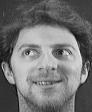
\includegraphics{Figures/Original}
         \caption{Original Image: \emph{s07/3.pgm}.}
     \end{subfigure}%
     \quad
     \begin{subfigure}[t]{0.45\textwidth}
         \centering
         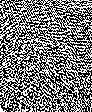
\includegraphics{Figures/Original-DCT}
         \caption{DCT applied to original image.}
     \end{subfigure}
    \caption{Original face and DCT applied to it.}
    \label{fig:ex1a}
\end{figure}

The image on the right is a representation of the image on the left. This representation si created using the \textbf{Discrete cosine transform}, that is, using sums of \emph{cosines}. There are a few different ways of expressing the DCT, but one of the most common ones is:
\[
 X_{k}=\sum _{n=0}^{N-1}x_{n}\cos \left[\,{\tfrac {\,\pi \,}{N}}\left(n+{\frac {1}{2}}\right)k\,\right]\qquad {\text{ for }}~k=0,\ \dots \ N-1
\]

\subsection{Using the original configuration parameters (\inline{train = 6} images, \inline{test = 4} images, DCT \inline{coefficients = 10}), plot the resulting DET image and indicate the resulting EER.}

We only have to let the whole \inline{FaceRecognition.m} script to execute. At the end, it plots the \emph{DET (Detection Error Trade-Off)} curve, which is a compromise between a False Rejection Rate (\emph{(FRR)}) and a False Acceptance Rate (\emph{FAR}). 

The \textbf{EER} is the point where \(FAR = FRR\), that is, the point where we accept the same percentage of false examples that we reject of positive examples. It is marked with a circle in Figure \ref{fig:ex1b}


\begin{figure}[H]
  \centering
  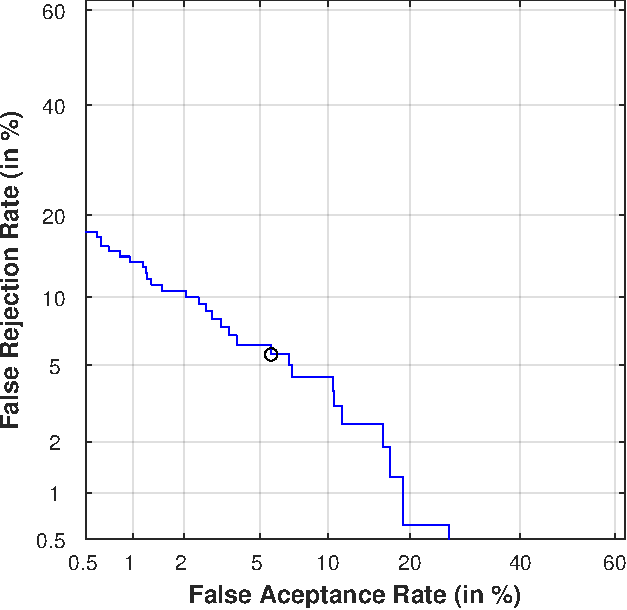
\includegraphics[scale=0.7]{Figures/EER-1}
    \caption{DET curve with marked EER.}
    \label{fig:ex1b}
\end{figure}

We can appreciate in Figure \ref{fig:ex1b} that the EER (circled) is around \(\sim 5.5\%\). Also, the code shows on screen that the EER is \inline{EER = 5.6571}.


\subsection{Find out the configuration of the DCT coefficients that achieves the best EER results (keeping train = 6 images, test = 4 images). Justify your result, including the resulting DET image and EER value.}

In this case where the number of images is small and the techniques that we apply to the image do not take long to execute, we can perform a \emph{grid search} varying the \emph{coefficients} parameter. We have done the following steps:

\begin{enumerate}

\item Extracted the important parts of the code file \inline{FaceRecognition.m} and introduced them in a new file (\inline{eer.m}) containing the function \inline{eer(n_train,n_test,param_coeff)} that, given the number of images used for train and test, and given a number of coefficients, computes the EER for those parameters.
  
\item We have created the script \inline{grid_search_coeff} that executes the code in \inline{eer.m} using the range \(\{1,\dots,20\}\) for the coefficients and saving the EER result in each case.

\item We plot the results in a chart, remarking the minimum. this is shown in Figure \ref{fig:ex1c}.
\end{enumerate}

\begin{figure}[H]
  \centering
  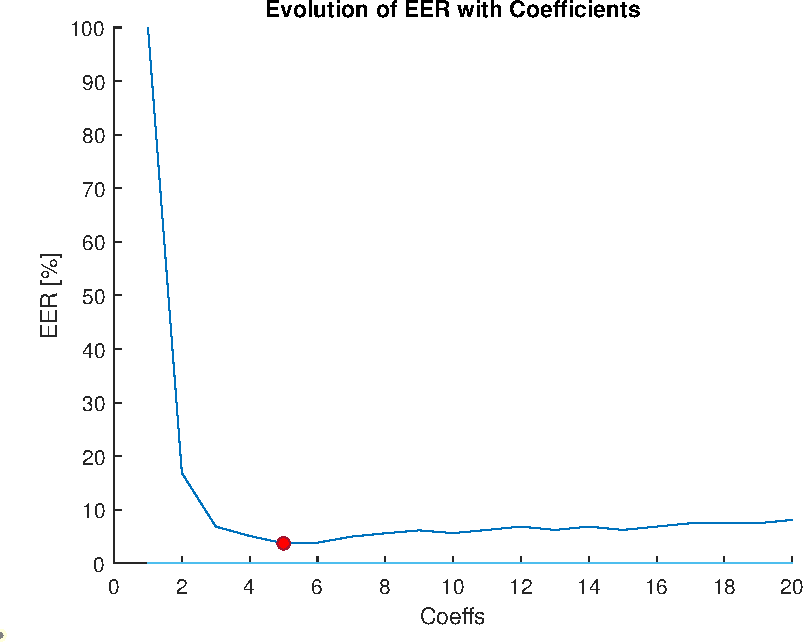
\includegraphics[scale=0.5]{Figures/EERvsCOEFF}
    \caption{Evolution of the EER with the number of coefficients.}
    \label{fig:ex1c}
\end{figure}


As we can see, the \textbf{optimal} number of coefficients is \(5\), obtaining an \(EER = 3.750\). We can appreciate how using a small number of coefficients, the EER is very high (the features are not captured). When using more than \(5\), the EER slowly starts to increase.


\subsection{ Once selected the best configuration of the DCT coefficients (in previous point), analyze the influence of the number of training images in the system performance. Include the EER result achieved for each case (from \(train = 1\) to \(train = 7\)). Justify the results.}


In this case, we can make good use of our previously defined function \inline{eer} and adapt the code in \inline{grid_search_coeff} to make it vary the parameter \inline{n_train} (and, thus, \inline{n_test} since \(n\_test = total - n\_train\)).

We create a new script called \inline{grid_search_ntrain} that uses \(n\_train = \{1,\dots,9\}\) and we run the script, obtaining the graph in Figure 

\begin{figure}[H]
  \centering
  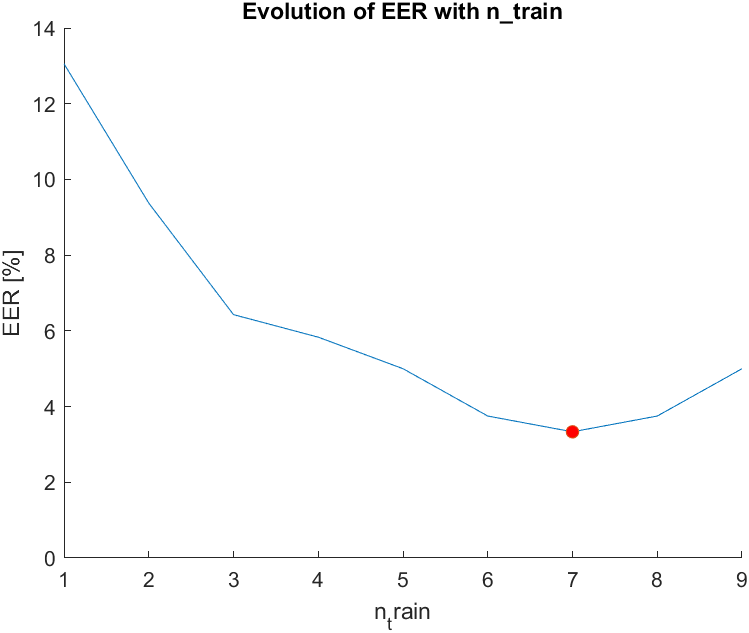
\includegraphics[scale=0.5]{Figures/EERvsNTRAIN}
    \caption{Evolution of the EER with the number of coefficients.}
    \label{fig:ex1d}
\end{figure}

The minimum value of the EER is obtained when we use \(n\_train = 7\) images, obtaining \(EER = 3.33\), which is a lower value than the one we obtained previously when we optimized the coefficients.\\ 


With this and the previous question, what we have done is typically called \textbf{grid search}, that is, searching for the best hyperparameters of our model. Usually, the number of images in train and test subsets is not an hyperparameter, since the quantity of available images is much higher, and a partition of \(70-75\%\) of the size is chosen for train and the rest for the test set. In this case, we reached that the train set has the \(70\%\) of the total size of our dataset. 

The results are positive, since we have searched for the combination that \textbf{optimizes} the EER in this particular problem. As a quick recall, the optimal parameters when we seek to \textbf{minimize the EER} are:
\begin{enumerate}
\item \(n\_train = 7, n\_test = 3\)
\item \(coefficients = 5\)
\end{enumerate}


\section{Task 2}
The goal of this task is to change the feature extraction module. Instead of using DCT coefficients as in Task 1, you must consider Principal Component Analysis (PCA) to extract more robust features. 
You can use the pca.m function available in Matlab. For the training phase, you should follow:
\begin{minted}{MatLab}
[coeff_PCA,MatrixTrainPCAFeats,latent] = pca(MatrixTrainFeats);
meanTrainMatrix=mean(MatrixTrainFeats);
\end{minted}
It is important to remark that the PCA function must be applied once for all training users and samples (not one PCA per user as this would provide specific \inline{coeff_PCA} parameters per user).  
For the test phase, you should follow:
\begin{quote}
For each test, subtract the meanTrainMatrix, and multiply by the \inline{coeff_PCA} transformation matrix in order to obtain the test features in the PCA domain.
\end{quote}
For more information, check Matlab Help: \url{https://es.mathworks.com/help/stats/pca.html}

\subsection*{Preparation}

\textbf{Note.-} The code of this preparation section can be found in the file \inline{PCA_EER.m}.\\

To begin with this task, we must adapt the code used before in order to change the way the feature extraction is done. We are told that we must apply PCA as it is usually done: to a \(M \in \mathcal M_{r \times c}\) matrix with \(r\) examples with \(c\) features per example. The idea is to reduce that matrix to another matrix \(M_{PC} \in \mathcal M_{r \times c'}\), where \(r' < r\), but keeping the most relevant information about each image.

Thus, we change the way we store the images, we now \emph{flatten} each of them into a single row to create the just mentioned \(M\) matrix. We declare in this case a Matrix of size \(Train\cdot 40 \times  (image\_length \cdot image\_width)\).

\begin{minted}{MatLab}
  size = length*width;
  %Initialize the Feature and Label Matrix for both train and test
  MatrixTrainFeats=zeros(Train*40,size); 
  MatrixTestFeats=zeros(Test*40,size); 
\end{minted}

Then, we have to flatten (convert each image matrix \(M \in \mathcal M_{r \times c}\) to a vector in \(\mathbb R^{r \cdot c}\), and introduce in the corresponding \emph{Train/Test Matrix}. We have slightly changed how the code of the original \inline{FaceRecognition.m} does this part, making it a little bit easier. The result is the following:

\begin{minted}{MatLab}
  for j=1:10
  im=imread(images(j).name);
  im=double(im);
  % Flatten image and add it to big matrix
  im_flat = reshape(im.',1,[]);

  %%%  Training Dataset
  if j <= Train
      MatrixTrainFeats((i-1)*Train + j, : ) = im_flat;
      MatrixTrainLabels((i-1)*Train + j, 1) = i;
  %%% Test dataset
  else
      MatrixTestFeats((i-1)*Test + (j - Train), : ) = im_flat;
      MatrixTestLabels((i-1)*Test + (j - Train), 1) = i;
  end
\end{minted}

Lastly, as we are indicated in the task, we have to extract the principal components of the matrix that contains the features of \textbf{all} the images, that is: \inline{MatrixTrainFeats}. The MatLab method \inline{pca} returns the mean \(\mu\) and the PCA coefficients, so we can use them to project the Test set into the feature space.
\begin{minted}{MatLab}
  % PCA on Training matrix
  [PCA_coeffs,MatrixTrainPCA,latent,none,explained,mu] = pca(MatrixTrainFeats);
  % Project Test Set
  MatrixTestPCA = (MatrixTestFeats - mu)*PCA_coeffs;  
\end{minted}

We remark the information contained in each of the returned variables from PCA:

\begin{itemize}
\item \inline{PCA_coeffs}\(\in \mathcal M_{p \times p}\) are the coefficients of the principal components.
\item \inline{MatrixTrainPCA} contains the representation of the original data in the principal component feature space.
\item \inline{latent} contains the  Hotelling's T-squared statistic for each observation in X.
\item \inline{explained} contains the percentage of the total variance explained by each principal component.
\item \inline{mu} contains the estimated mean of each variable in the original data.
\end{itemize}

The distance computation used in \inline{FaceRecognition.m} is kept, so we do not modify it. We are now ready to perform the required sub-tasks.

\subsection{ Using the parameters \(train = 6\) and \(test = 4\), paste the DET curve and indicate the EER when using all the PCA components.}


Using the previously commented code, we run the \inline{PCA_EER} script with the mentioned sizes for train and test subsets and obtain the DET curve plotted in Figure \ref{fig:ex2a}. In this subtask, we use \textbf{all components} obtained by PCA.

\begin{figure}[H]
  \centering
  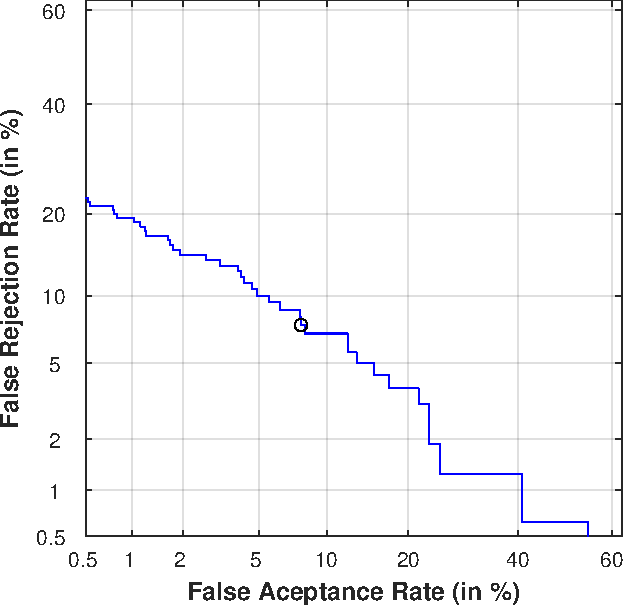
\includegraphics[scale=0.7]{Figures/PCA-1-EER}
    \caption{DET curve for PCA with \(n\_train = 6\) and \(n\_test = 4\), using \textbf{all components}.}
    \label{fig:ex2a}
\end{figure}

We obtain an \(EER = 8.125\), which is approximately \(2.5 \%\) higher than the one we obtained in the simplest case using the DCT. Using all the components returned from PCA is not the best option.



\subsection{ A key aspect for the PCA is the number of components considered. Analyze and represent how the EER value changes in terms of the number of PCA components. Give your explanation about the results achieved.}

As we already know, we obtain the principal components by diagonalizing the covariance matrix of the data. This way, we obtain principal directions \(v_1,\dots, v_n\) and eigenvalues \(\lambda_1,\dots,\lambda_n\), which indicate the \textbf{percentage} of the variance explained by each component. The components are sorted by the variance explained (its eigenvalue \(\lambda_i\). The most common technique when using PCA is \textbf{selecting} a number of components that explain a decent amount of the variance. \\

In order to determine how many components we want to select, let us first do an analysis of the variance explained. We find (by obtaining the number of elements of the variable \inline{explained}) that PCA returns \(239\) components. Let us show in Figure \ref{fig:ex2b}  the percentage of variance explained by each of them and the accumulated variance explained by the components \(1,\dots, i\) for each \(i = 1,\dots, 239\). 

\begin{figure}[H]
  \centering
       \begin{subfigure}[t]{0.45\textwidth}
         \centering
         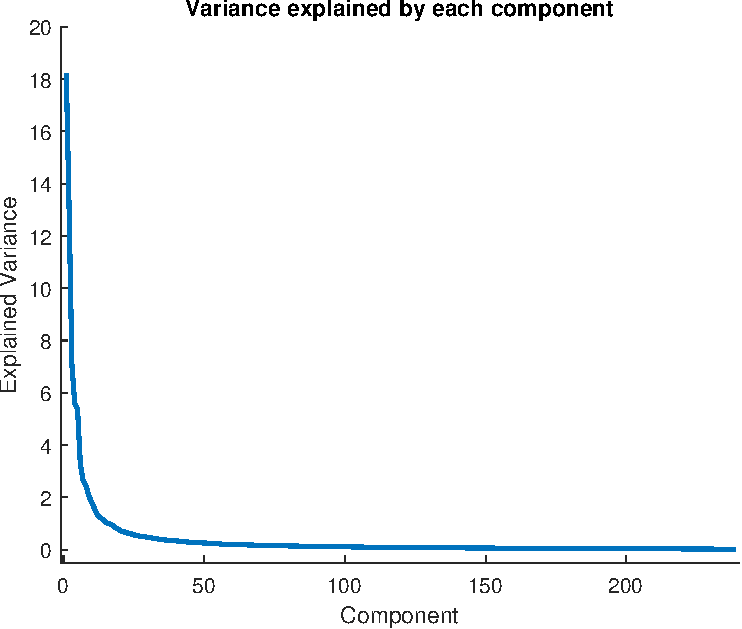
\includegraphics[scale=0.6]{Figures/VariancePerComponent}
         \caption{Variance explained by each component.}
     \end{subfigure}%
     \quad
     \begin{subfigure}[t]{0.45\textwidth}
         \centering
         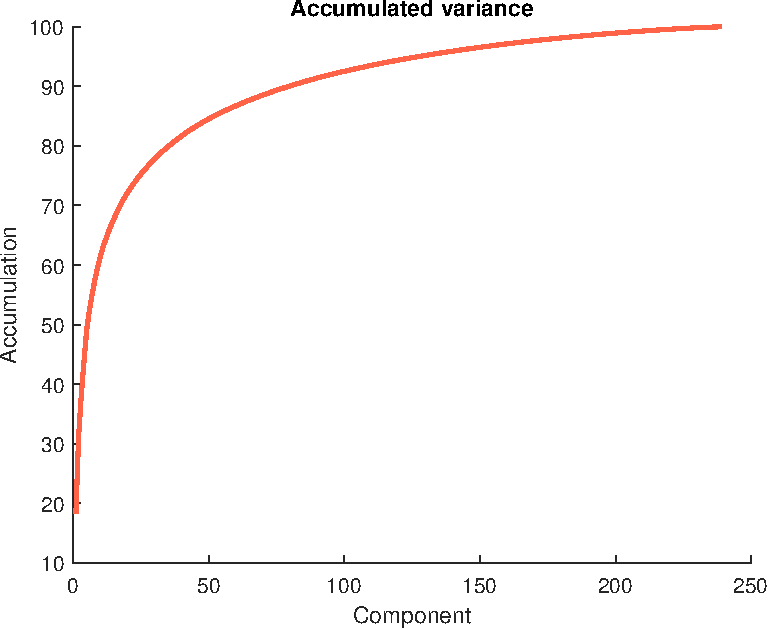
\includegraphics[scale=0.6]{Figures/accumulated_variance}
         \caption{Accumulated variance explained.}
     \end{subfigure}
    \caption{Explained variance representations.}
    \label{fig:ex2b}
\end{figure}

We can observe in the graphics that using approximately \(50\) components we are explaining \(\approx 80\%\) of the total variance, which is usually enough to be able to classify the images well. Also, from the component \(50\) onwards, the components explain less than \(1\%\) of the total variance, which means that they are possibly not really relevant.\\

We now compute the EER for each number of components. We create a fragment of code that \emph{iterates} over all the possible number of components (\(1\) to \(239\)) and computes the EER for each of them, and gets the number of components which results in a smaller EER. The result is shown in Figure \ref{fig:ex2c}.


\begin{figure}[H]
  \centering
  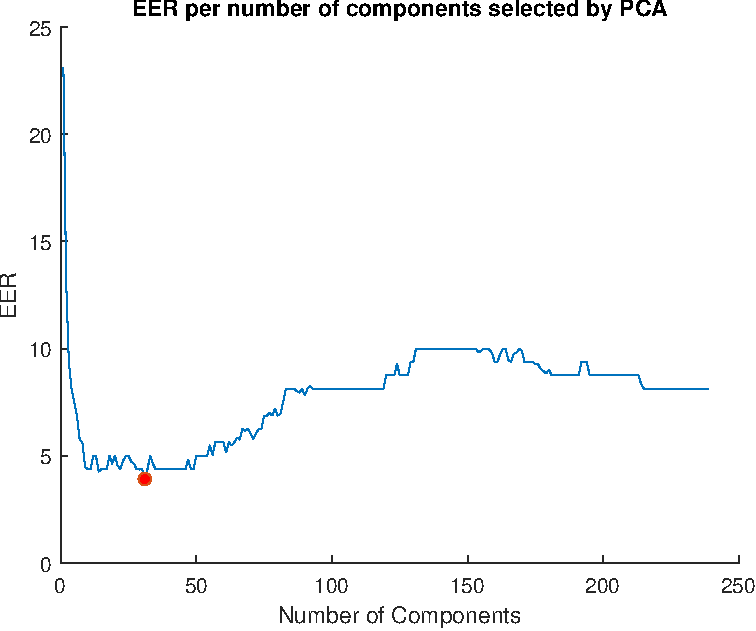
\includegraphics[scale=0.7]{Figures/ERR-per-ncomponents}
    \caption{EER obtained using each possible number of components returned by PCA.}
    \label{fig:ex2c}
\end{figure}


As we can observe, using less than \(50\) components (which is the number of components that can explain approximately \(80\%\) of the variance), results in the lowest values of the EER. The EER increases when we increment the number of components, and this \textbf{makes sense}, since we have already mentioned that after the \(50-\)th component, the rest of them explain less than \(1\%\) of the variance, which means that they are \textbf{not significant}. \\

All in all, our results in terms of the EER are coincident with our preliminary study of the explained variance by the components.




\subsection{ Indicate the optimal number of PCA components and paste the resulting DET curve together with the EER achieved. Compare the results using PCA with the DCT features considered in Task 1.}

After the loop that iterates through all possible components, we added some code that outputs the minimum of the computed EERs. This code outputs the following:

\begin{minted}{MatLab}
  Min EER is obtained with 31 components
  Minimum EER is  3.910256e+00 
  Explained Variance 7.826086e+01
\end{minted}

As we can see, we obtain that selecting \textbf{31 components} results in \(EER = 3.91\), which is the minimum that we can obtain using PCA. Also, we are explaining approximately a \(78\%\) of the total variance, which is quite a high quantity. We \textbf{state} that the optimal number of PCA components to use in this problem is \(31\). The resulting DET curve is plotted in Figure \ref{fig:ex2c-optim}.

\begin{figure}[H]
  \centering
  \includegraphics[scale=0.7]{Figures/DET-optim-comps-PCA}
    \caption{DET curve for \(n\_components = 31\) in PCA feature selection.}
    \label{fig:ex2c-optim}
\end{figure}

\subsubsection{Comparison with the previous method}

Now we want to compare the results obtained using PCA with the results obtained using the feature extractor that used the DCT. For PCA we used a fixed \(n\_train = 6\) and \(n\_test = 4\). Remember that, in the DCT method, the best results were achieved using \(n\_train = 7, n\_test = 3\). However, we have tested this configuration (and also \(n\_train = n\_test = 5\)) in the PCA feature extraction, but the results have only gotten worse (we obtained higher values for the EER).

With this in consideration, we have resumed all the information until this point in Table \ref{table:comp1}. For each of the feature extraction methods, we include the original hyperparameters and the optimal hyperparameters selection.

\begin{table}[H]
  \centering
  \begin{tabular}{l|rr}
  Method/Hyperparameters                                                & \multicolumn{1}{l}{Starting} & \multicolumn{1}{l}{Best} \\ \hline
  \begin{tabular}[c]{@{}l@{}}DCT\end{tabular} & $5.5$                        & $3.33$                   \\
  PCA                                                                   & $8.125$                      & $3.91$                  
  \end{tabular}
  \caption{Comparison of the results obtained with both used methods.}
  \label{table:comp1}
  \end{table}

PCA obtains an EER \(0.6 \%\) higher than the one obtained by using the DCT, which is worse than the first case but not really in a determinant quantity. However, we know that PCA focus on explaining the variance of the data, so the extracted features might be more relevant when generalizing this code for a larger dataset, so we would \textbf{choose PCA} as the most relevant way of extracting features.



\section{Extra Task}

The goal of this task is to improve the matching module. Instead of using a simple distance comparison, you must consider Support Vector Machines (SVM). In this case, you should train one specific SVM model per user using the training data (train = 6 images).
Features extracted using the PCA module developed in Task 2 must be considered in this Task. 
You can use the fitcsvm function available in Matlab. For the training phase, you should follow:
\begin{minted}{MatLab}
SVMModel = fitcsvm(…)
\end{minted}
For the test phase, you should follow:
\begin{minted}{MatLab}
[label,score]= predict(SVMModel,MatrixTestFeats);
\end{minted}
to obtain the scores for each user model. 
For more information, check Matlab Help:
\url{https://es.mathworks.com/help/stats/fitcsvm.html?lang=en} 

\subsection{Introduction}

In this last task, we use the PCA feature extractor created in the last task to apply an \emph{Support Vector Machine} to the extracted features and compute the EER using the predictions given by this SVM.\\

We will use the \textbf{one versus all} strategy, that is: consider for each class a binary classification problem where the positive examples are the ones belonging to that class and the rest of the elements in the dataset will be negative examples.The code for this task will be in the module \inline{PCA_SVM.m}. However, in order to make it simpler, we create a submodule called \inline{compute_eer_svm} that receives the Train and Test sets (and a few extra parameters) and returns the EER for the given sets.\\

As we executed the train stage for the first time, we realized that the training times were \textbf{quite high}. To avoid this problem, we found the MatLab tool \inline{Parallel Computing Toolbox}, which allows us to \textbf{parallelize} the executions of the training of the multiple classifiers for a determined number of features. 

We can divide the code of the script \inline{compute_eer_svm} in two main sections. The \textbf{first one} trains an SVM (using a given kernel) for each of the individuals of the dataset (we use \inline{parfor} to parallelize the for loop)

\begin{minted}{MatLab}
  parfor i = 1:n_users
    idx = y_train == i;

    if strcmp(kernel_type,'polynomial')
        SVMModels{i} = fitcsvm(X_train,idx, ...
            "KernelFunction",kernel_type, ...
            "PolynomialOrder",degree, ...
            "Standardize",true);
    elseif strcmp(kernel_type,'rbf')
        SVMModels{i} = fitcsvm(X_train,idx, ...
            "KernelFunction",kernel_type, ...
            "KernelScale",scale);
    else % linear case
        SVMModels{i} = fitcsvm(X_train,idx);
    end
end
\end{minted}

Then, the second part predicts the test images for all the users and saves the scores to vectors using a mask that contains the true labels of the images. Lastly, our old friend \inline{Eval_Det} is called to compute the EER(and draw the DET curve).

\begin{minted}{MatLab}
parfor i=1:n_users  % For each user
    % Predict 
    [none , scores]=predict(SVMModels{i}, X_test);

    % Create a Mask to determine TargetScores
    userLabels = y_test(:, 1) == i;
    % Apply Positive and negative masks to obtain Scores vectors
    TargetScores=[TargetScores, scores(userLabels, 2)'];
    NonTargetScores=[NonTargetScores, scores(~userLabels, 2)'];
end

[EER] = Eval_Det(TargetScores, NonTargetScores, 'b', plot_eer);
\end{minted}


\subsection{ Using the parameters train = 6 and test = 4, paste the DET curves and indicate the EERs in the following cases: 1) regarding the KernelFunction parameter of the SVM (using all PCA components), and 2) regarding the number of PCA components considered for the feature extraction module (using the KernelFunction polynomial and starting with 3 PCA components).}

\subsubsection{Using the KernelFunction}

One of the arguments of the previously mentioned script \inline{compute_eer_svm} is the \textbf{kernel function}. A kernel is a non-negative real-valued and integrable function \(K\), used to perform a transformations of the features to a different feature space. In this case, we will try three different kernels applied to the features obtained by PCA:

\begin{itemize}
\item Linear kernel: the default kernel, which can be expressed as
\[
K(x,y) = x^T y.  
\]
\item Polynomial kernel: A degree-\(d\) polynomial kernel is defined as
\[
K(x,y) = (x^T y + c)^d.  
\]
In our case, we tried with \(d = 2\). When we use this kernel, we use \inline{standardize = true} since it provides better results and the training is faster.
\item Gaussian (or RBF) kernel, which has the following expression:
\[
K(x,y) = exp(-\gamma \lVert x- y \rVert^2).  
\]
This is the most common kernel, since it provides very good results in a wide variety of classification and regression problems.
\end{itemize}

After executing our code with the three kernels, we obtained the results shown in Table \ref{table:extra}

\begin{table}[H]
  \centering
  \begin{tabular}{l|lll}
      & Linear                      & Polynomial                & Gaussian                  \\ \hline
  EER & \multicolumn{1}{r}{$3.125$} & \multicolumn{1}{r}{$7.5$} & \multicolumn{1}{r}{$2.5$}
  \end{tabular}
  \caption{EERs for each of the kernels using all PCA components.}
  \label{table:extra}
  \end{table}

  We also plot the DET curve for each of the different kernels in Figure \ref{fig:extra:all}.

  \begin{figure}[H]
    \centering
         \begin{subfigure}[t]{0.32\textwidth}
           \centering
           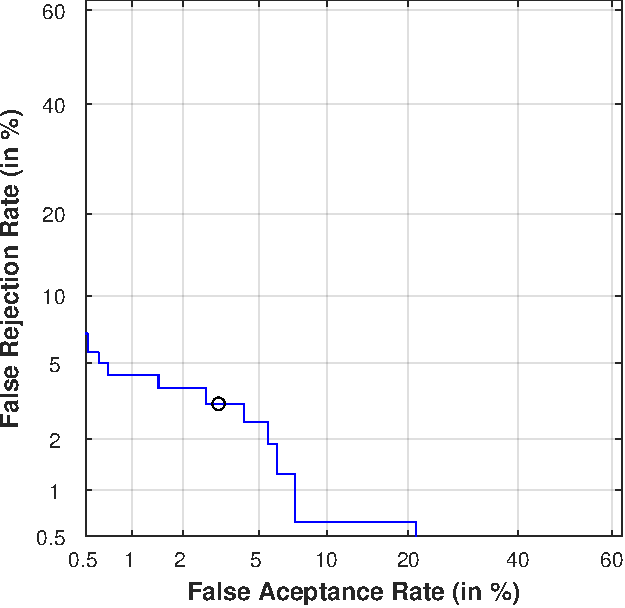
\includegraphics[scale=0.4]{Figures/SVM-Linear}
           \caption{Linear}
       \end{subfigure}%
       \quad
       \begin{subfigure}[t]{0.32\textwidth}
           \centering
           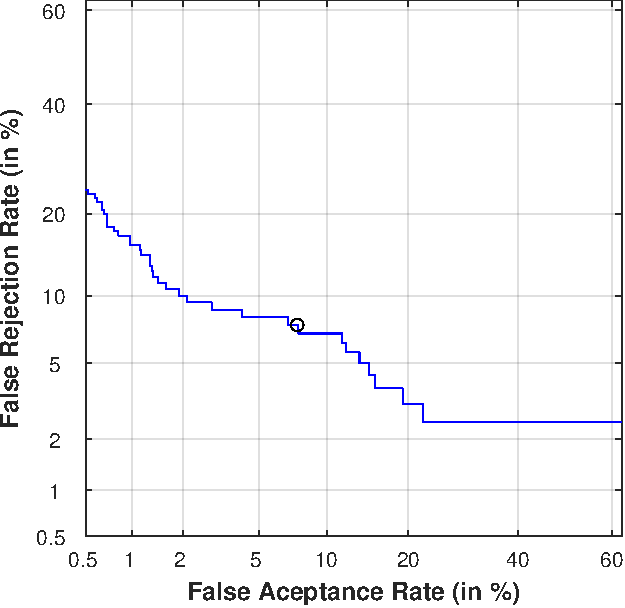
\includegraphics[scale=0.4]{Figures/SVM-POLY}
           \caption{Polynomial.}
       \end{subfigure}
       \quad
       \begin{subfigure}[t]{0.32\textwidth}
        \centering
        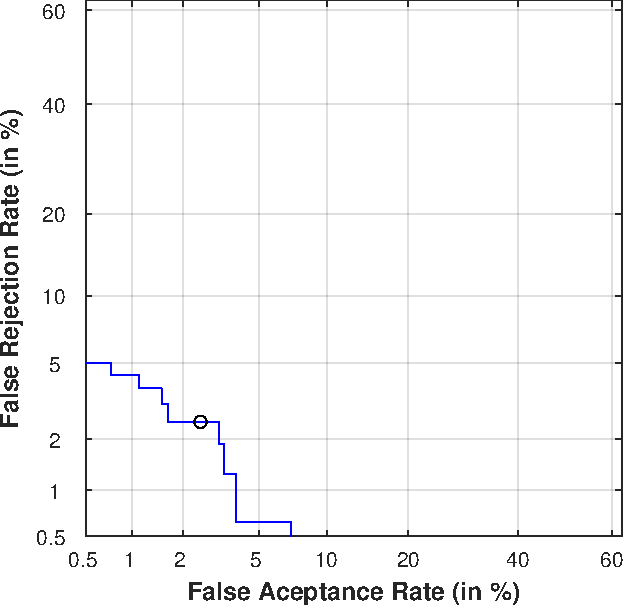
\includegraphics[scale=0.4]{Figures/SVM-RBF}
        \caption{RBF.}
    \end{subfigure}%
      \caption{DET curve for the different kernels.}
      \label{fig:extra:all}
  \end{figure}

As we can see in both the table and the DET curve, the \textbf{RBF kernel} is the one that performs better in terms of the EER metric, obtaining a \(2.5\%\) of EER when using all features extracted by PCA. This is already a really low percentage of equal error rate, which would result in a highly accurate classifier. The linear kernel also obtains a relatively low EER, being less than \(1\%\) above the RBF kernel, but also being \textbf{much slower} to train. Lastly, the Polynomial kernel is quite behind on this metric compared with RBF and Linear. Further experimentation with the degree \(d\) of the polynomial should be done to seek for a better-performing model using this kernel.\\


\begin{table}[H]
  \centering
  \begin{tabular}{l|r}
  Matcher  & \multicolumn{1}{l}{Lowest EER} \\ \hline
  Original & $3.33$                         \\
  SVM      & $2.5$                         
  \end{tabular}
  \caption{Comparison of minimum EERs obtained by each matcher.}
  \label{table:extra:comp}
  \end{table}

In Table \ref{table:extra:comp} we show the minimum EER obtained by each of the matchers tested. We find that training an SVM with an appropriate kernel over the extracted features is \textbf{better} than using the original matcher. 

\subsubsection{Changing the number of selected PCA components}

\emph{In this part of the task we realized that we needed to parallelize the executions}.\\

In the last subtask, we used \textbf{all the features} extracted by PCA. However, we already found out in previous tasks that using a much lower number of features provided in fact better results, since many features extracted by PCA are often of low importance.

In this last task, we would like to \textbf{vary the number of used features} and train an SVM over each of the possible number of features extracted to see which is the optimal number of features to use.

Although only the polynomial kernel was asked, we executed the code with the three kernels as extra. We will present the results one by one:

\begin{enumerate}

\item Polynomial.\\

Changing the number of used components was very beneficial for the polynomial kernel.
\begin{minted}{MatLab}
  Elapsed time is 88.666707 seconds.
  Min EER is obtained with 36 components
  Minimum EER is  1.939103e+00 
\end{minted}
The EER was reduced from \(7.5\) to \(1.93\), which is a really low value, indicating a very good model in general. Also, the elapsed time checking on all the possible components was less than one and a half minutes, which is quite fast. The \textbf{selected number of components} was 36, which is quite similar to the number of components found in previous task (remember that from component $\approx 50$, the rest of them do not explain more than \(1\%\) of the variance of the data.

\begin{figure}[H]
  \centering
       \begin{subfigure}[t]{0.45\textwidth}
         \centering
         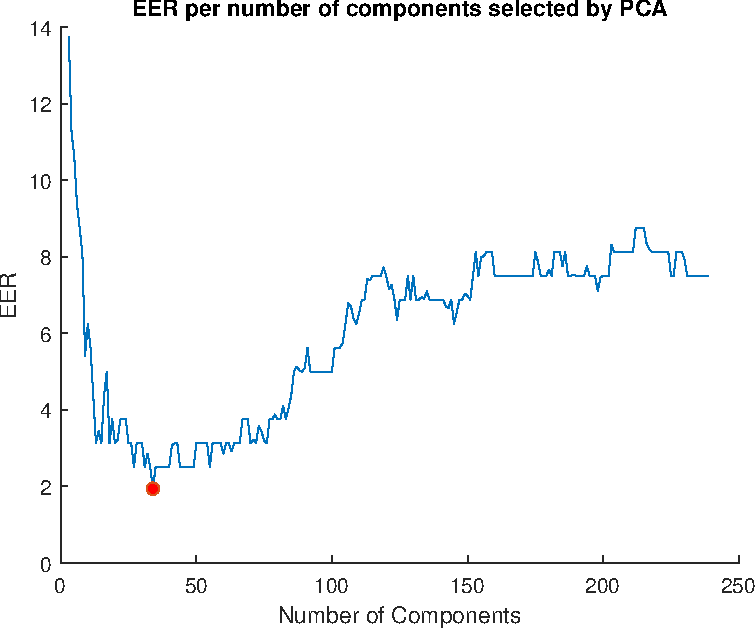
\includegraphics[scale=0.5]{Figures/SVM-POLY-1TOMAX}
         \caption{EER Evolution.}
     \end{subfigure}%
     \quad
     \begin{subfigure}[t]{0.45\textwidth}
         \centering
         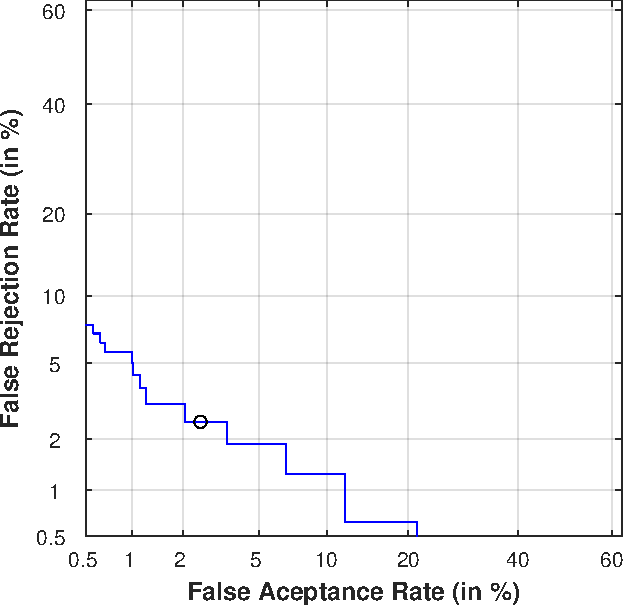
\includegraphics[scale=0.5]{Figures/SVM-POLY-OPTIMPCA}
         \caption{DET curve for SVM in \(36\) components.}
     \end{subfigure}
    \caption{Results for exploration with \textbf{polynomial kernel}.}
    \label{fig:extra:poly:all}
\end{figure}

The graph in Figure \ref{fig:extra:poly:all} shows that using this kernel, the components that explain most part of the variance obtain better results in terms of the EER, and when non-relevant components are added, the results get worse.

\item RBF.\\

This kernel was the fastest on training, obtaining very good results.
\begin{minted}{MatLab}
  Elapsed time is 80.869806 seconds.
  Min EER is obtained with 14 components
  Minimum EER is  1.875000e+00
\end{minted}

We can see that a very low number (14) of features are selected, obtaining \textbf{better results}(lower EER) than the ones obtained with the previous kernel.
\begin{figure}[H]
  \centering
       \begin{subfigure}[t]{0.45\textwidth}
         \centering
         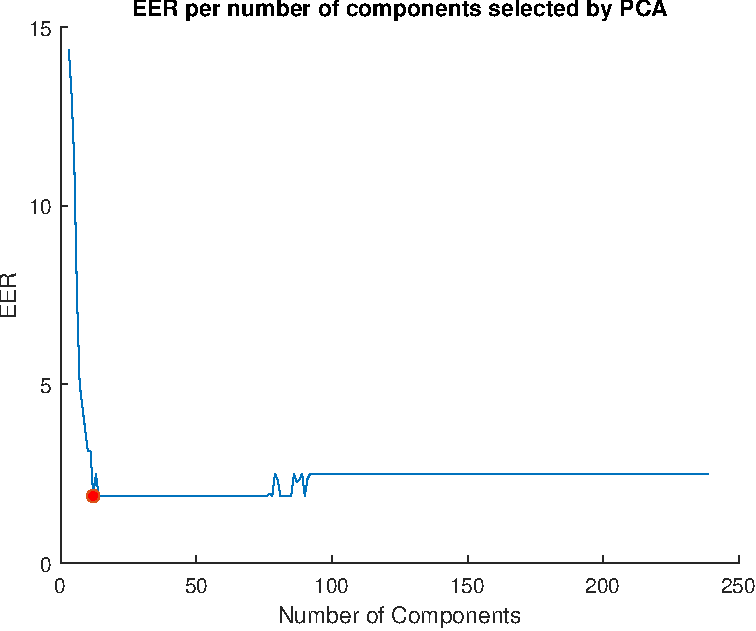
\includegraphics[scale=0.5]{Figures/SVM-RBF-1TOMAX}
         \caption{EER Evolution.}
     \end{subfigure}%
     \quad
     \begin{subfigure}[t]{0.45\textwidth}
         \centering
         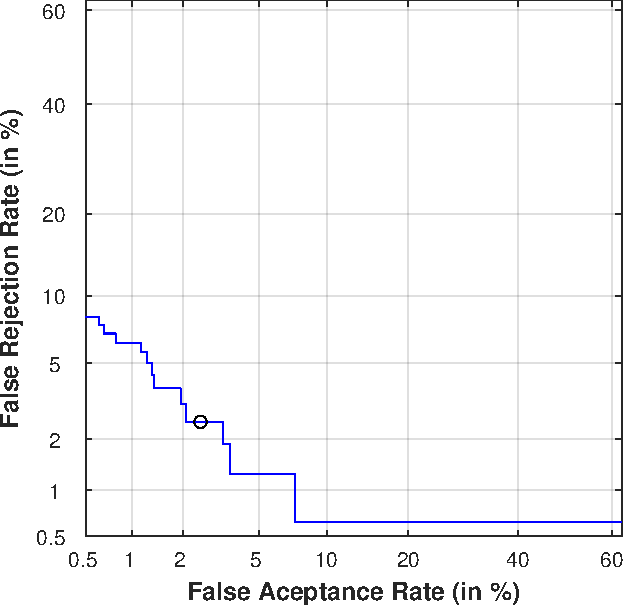
\includegraphics[scale=0.5]{Figures/SVM-RBF-OPTIMPCA}
         \caption{DET curve for SVM in \(14\) components.}
     \end{subfigure}
    \caption{Results for exploration with \textbf{RBF kernel}.}
    \label{fig:extra:rbf:all}
\end{figure}

Figure \ref{fig:extra:rbf:all} shows that using this kernel, there is a huge drop in the EER when we increment the number of considered features up to \(15\), but then the EER remains constant for any number of components that we add.

\item Linear.\\

This was the \textbf{slowest} of the three kernels trained. However,
\begin{minted}{MatLab}
  Elapsed time is 2079.385995 seconds.
  Min EER is obtained with 95 components
  Minimum EER is  1.666667e+00 
\end{minted}
our code shows that the linear kernel obtains \textbf{the lowest} EER obtained by any possible model until now. It uses, though, a quite high number of components, and the training time makes the use of this kernel \textbf{infeasible}.
\begin{figure}[H]
  \centering
       \begin{subfigure}[t]{0.45\textwidth}
         \centering
         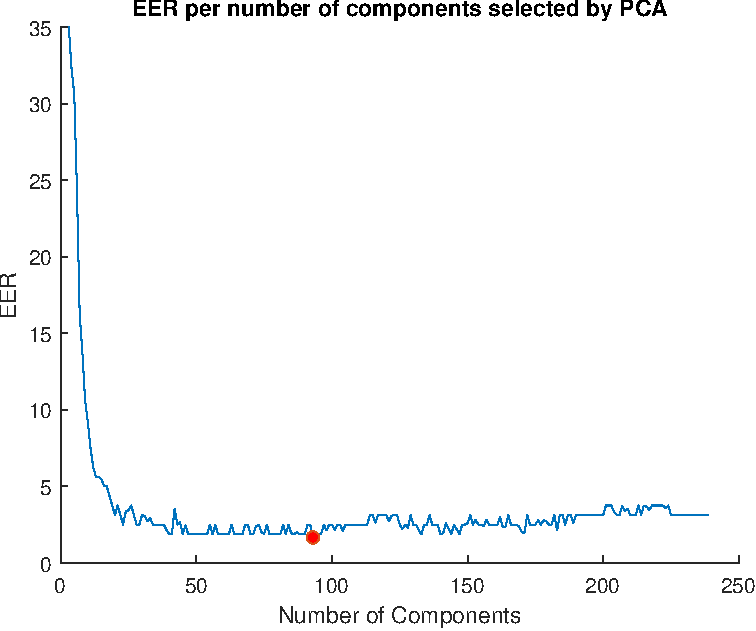
\includegraphics[scale=0.5]{Figures/SVM-Linear-1TOMAX}
         \caption{EER Evolution.}
     \end{subfigure}%
     \quad
     \begin{subfigure}[t]{0.45\textwidth}
         \centering
         \includegraphics[scale=0.5]{Figures/SVM-linear-OPTIMPCA}
         \caption{DET curve for SVM in \(95\) components.}
     \end{subfigure}
    \caption{Results for exploration with \textbf{linear kernel}.}
    \label{fig:extra:linear:all}
\end{figure}

Figure \ref{fig:extra:linear:all} reveals that the behavior of this kernel in terms of the EER per number of components is \emph{similar} to the behavior of the RBF kernel, although this one increases (very slowly) and seems like much less robust (lots of variations).

\end{enumerate}


\section{Conclusions}

In this assignment, we have verified that in the \textbf{Face Recognition} task (without using the \emph{state of art} Convolutional Neural Networks), there are a few aspects that must be researched to obtain a good classifier:

\begin{enumerate}
\item The \textbf{feature extractor} is very important and determines the quality of the final classifier. In this case, PCA outperformed the DCT feature extractor. There are, however, many other ways of extracting features from a face (and from an image in general) and many other methods should be studied for any particular problem.

\item The \textbf{matching engine} is also crucial and we have checked (as we all could expect) that the most intelligent idea is to train a classifier on top of the extracted features. We have also learned that seeking for a good \textbf{set of hyperparameters} (including the kernel) of the classifier determines the final performance of our classifier.
\end{enumerate}













\end{document}